\documentclass[9pt,t]{beamer}
% note that full page width is 12.8 cm and height is 9.6 cm

\mode<presentation>
{
  \usepackage[headline,footline]{beamerthemelectures}

}

% load packages
\usepackage[english]{babel}
\usepackage{graphicx}
\usepackage{multimedia}
%\usepackage[T1]{fontenc}
\usepackage{lmodern}
\usepackage{amsmath,amssymb}
\usepackage{pgf,booktabs,verbatim}
\usepackage{pgfarrows,pgfnodes}
\usepackage[absolute,overlay]{textpos}
\setlength{\TPHorizModule}{\paperwidth}
\setlength{\TPVertModule}{\paperheight}
\usepackage{tikz}

\setbeamertemplate{frametitle}{
\begin{centering}
\insertframetitle
\par
\end{centering}
} 

% create command to add nice looking citation
\newcommand{\reference}[1]{\flushright \vspace{-0.3cm} {\tiny #1}} 


\title{Solutions to Modeling Exercise \#6\\ The rock cycle}

\begin{document}

\section{}

%%%
\frame{
    \frametitle{\vspace{1cm}\huge The rock cycle}
   
}

\frame{
\frametitle{1a. Perturb continental igneous rock}
\begin{figure}
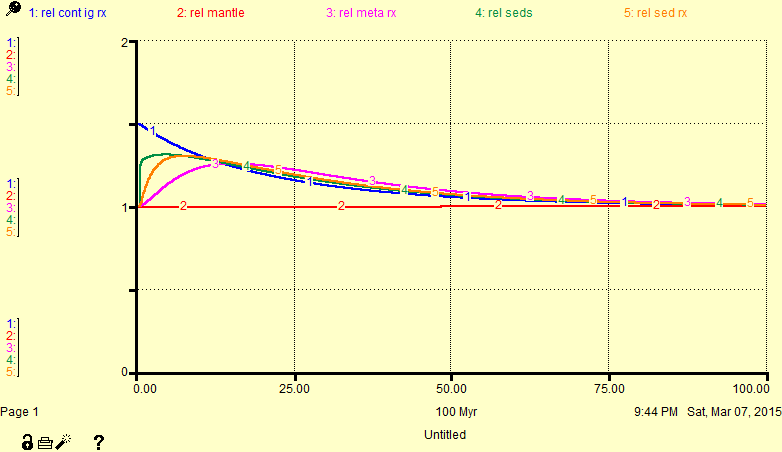
\includegraphics[width=0.9\textwidth]{./p1a.jpg}
\end{figure}
\begin{itemize}
\item 
\end{itemize}
}

\frame{
\frametitle{1a. Perturb continental igneous rock}
\begin{figure}
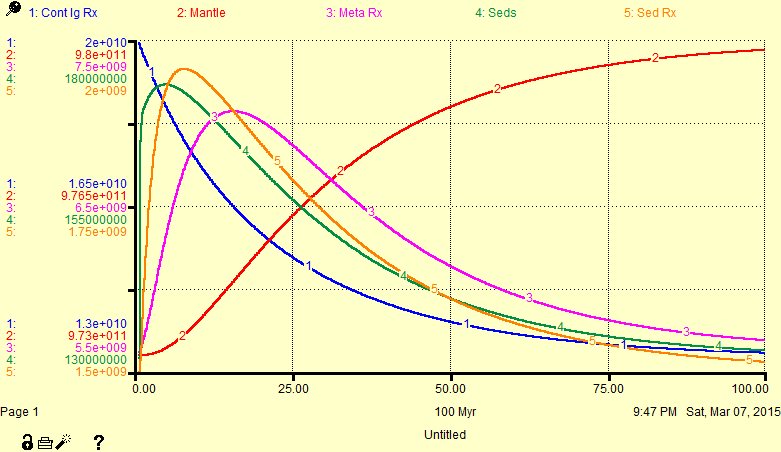
\includegraphics[width=0.9\textwidth]{./p1b.jpg}
\end{figure}
\begin{itemize}
\item 
\end{itemize}
}

\frame{
\frametitle{1b. Increase weathering rate}
\begin{figure}
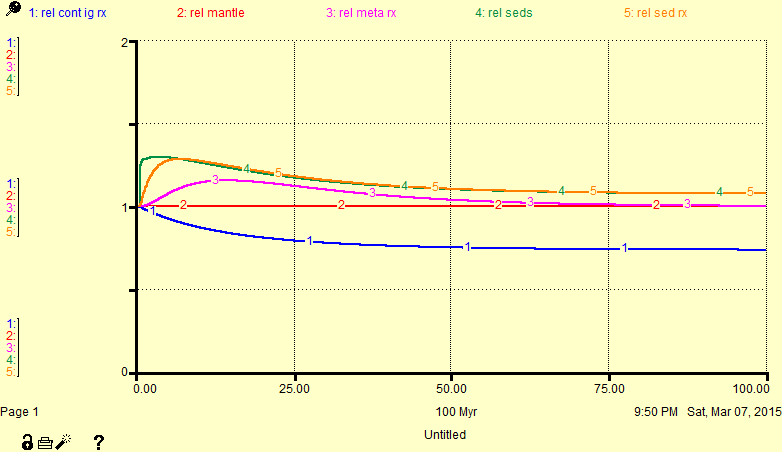
\includegraphics[width=0.9\textwidth]{./p1c.jpg}
\end{figure}
\begin{itemize}
\item 
\end{itemize}
}

\frame{
\frametitle{1b. Increase weathering rate}
\begin{figure}
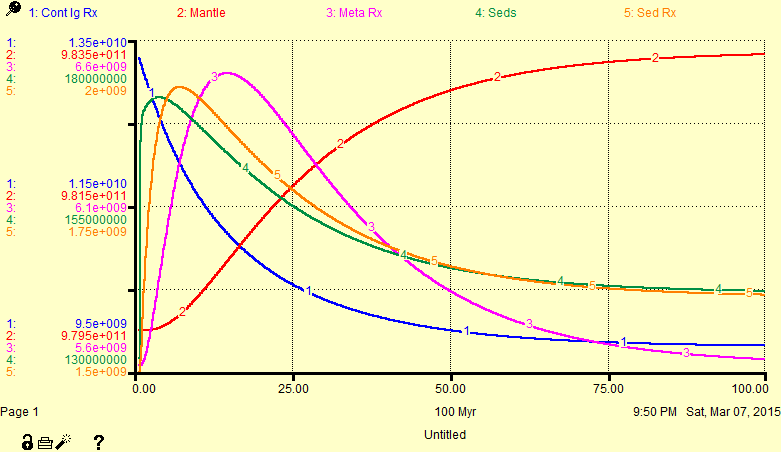
\includegraphics[width=0.9\textwidth]{./p1d.jpg}
\end{figure}
\begin{itemize}
\item 
\end{itemize}
}

\frame{
\frametitle{2. Formation of the early Earth}
\begin{figure}
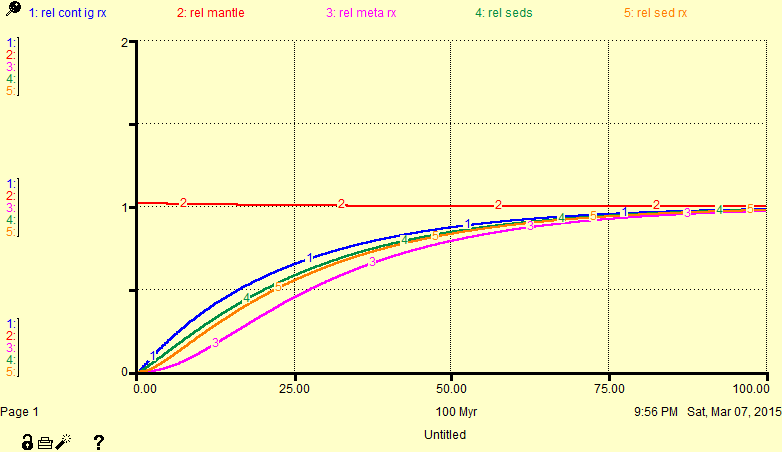
\includegraphics[width=0.9\textwidth]{./p2a.jpg}
\end{figure}
\begin{itemize}
\item 
\end{itemize}
}

\frame{
\frametitle{3a. High tectonic activity early in Earth's history}
\begin{figure}
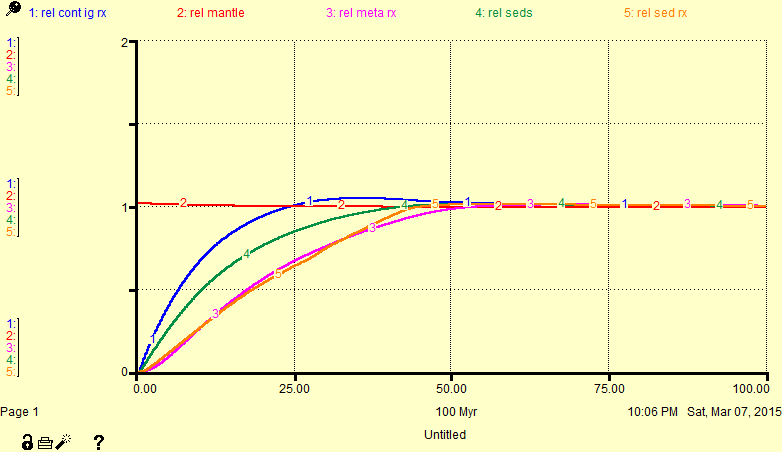
\includegraphics[width=0.9\textwidth]{./p3a.jpg}
\end{figure}
\begin{itemize}
\item 
\end{itemize}
}

\frame{
\frametitle{3a. High tectonic activity early in Earth's history}
\begin{figure}
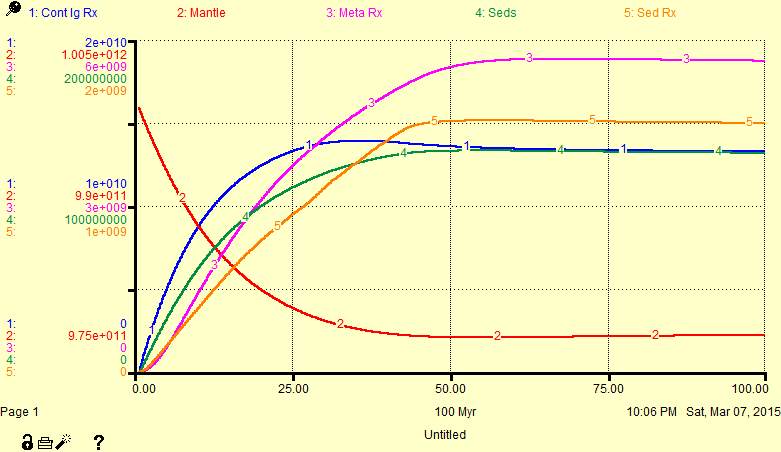
\includegraphics[width=0.9\textwidth]{./p3b.jpg}
\end{figure}
\begin{itemize}
\item 
\end{itemize}
}

\frame{
\frametitle{3b. Sinusoidal variations in tectonic activity}
\begin{figure}
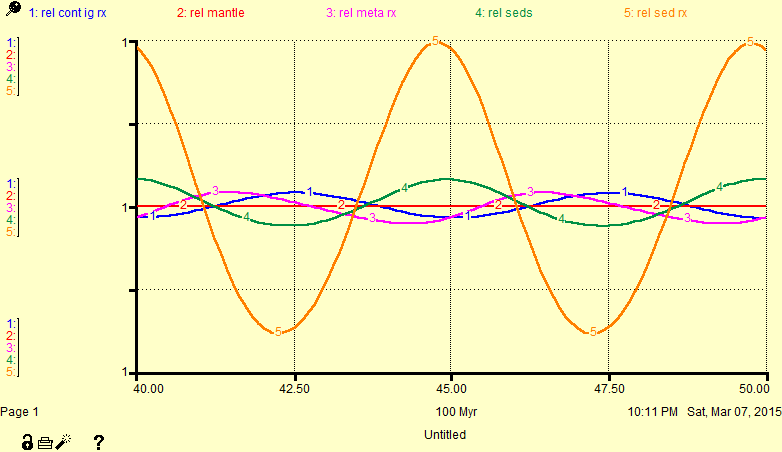
\includegraphics[width=0.9\textwidth]{./p3c.jpg}
\end{figure}
\begin{itemize}
\item 
\end{itemize}
}

\frame{
\frametitle{3b. Sinusoidal variations in tectonic activity}
\begin{figure}
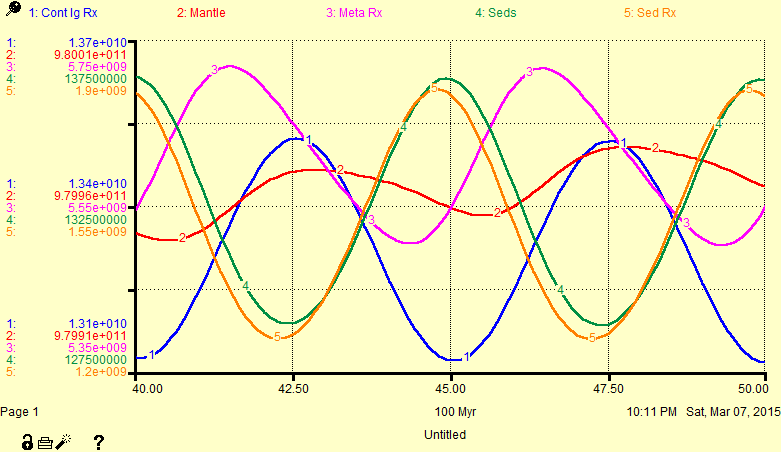
\includegraphics[width=0.9\textwidth]{./p3d.jpg}
\end{figure}
\begin{itemize}
\item
\end{itemize}
}

\end{document}

\frame{
\frametitle{Key ideas}
\begin{itemize}
\item System parameters can vary unpredictably as a system evolves toward a steady-state
\item The initial conditions matter $\rightarrow$ systems often have multiple steady states; the initial conditions determine which steady state a system will approach
\item Short pertubations can cause a ``permanent'' transition from one state to another
\item Observed a transition out of the (i) cold state for large perturbations in temperature (ii) warm state for moderate perturbations in temperature
\item Also produced transitions from one state to another by modifying the salinity difference
\end{itemize}
}

\end{document}
